%%%%%%%%%%%%%%%%%%%%%%%%%%%%%%%%%%%%%%%%%%%%%%%%%%%%%%%%%%%%%%%%%%%%%%%%%%
%
% Plantilla para libro de texto de matemáticas.
%
% Esta plantilla ha sido desarrollada desde cero, pero utiliza algunas partes
% del código de la plantilla original utilizada en apuntesDGIIM
% (https://github.com/libreim/apuntesDGIIM), basada a su vez en las plantillas
% 'Short Sectioned Assignment' de Frits Wenneker (http://www.howtotex.com),
% 'Plantilla de Trabajo' de Mario Román y 'Plantilla básica de Latex en Español'
% de Andrés Herrera Poyatos (https://github.com/andreshp). También recoge
% ideas de la plantilla 'Multi-Purpose Large Font Title Page' de
% Frits Wenneker y Vel (vel@latextemplates.com).
%
% Licencia:	
% CC BY-NC-SA 4.0 (https://creativecommons.org/licenses/by-nc-sa/4.0/)
%
%%%%%%%%%%%%%%%%%%%%%%%%%%%%%%%%%%%%%%%%%%%%%%%%%%%%%%%%%%%%%%%%%%%%%%%%%

% ---------------------------------------------------------------------------
% CONFIGURACIÓN BÁSICA DEL DOCUMENTO
% ---------------------------------------------------------------------------

%\documentclass[11pt, a4paper, twoside]{article} % Usar para imprimir
\documentclass[10pt, a4paper]{article}

\linespread{1.3}            % Espaciado entre líneas.
\setlength\parindent{0pt}   % No indentar el texto por defecto.
\setlength\parskip{7pt}

% ---------------------------------------------------------------------------
% PAQUETES BÁSICOS
% ---------------------------------------------------------------------------

% IDIOMA
\usepackage[utf8]{inputenc}
\usepackage[spanish, es-tabla, es-lcroman, es-noquoting]{babel}
\usepackage[table,xcdraw]{xcolor}

% MATEMÁTICAS
\usepackage{amsmath}    % Paquete básico de matemáticas
\usepackage{amsthm}     % Teoremas
\usepackage{mathrsfs}   % Fuente para ciertas letras utilizadas en matemáticas

% FUENTES
\usepackage{newpxtext, newpxmath}   % Fuente similar a Palatino
\usepackage{FiraSans}                 % Fuente sans serif
\usepackage[T1]{fontenc}
\usepackage[italic]{mathastext}     % Utiliza la fuente del documento
                                    % en los entornos matemáticos

% MÁRGENES
\usepackage[margin=2.5cm, top=3cm]{geometry}

% LISTAS
\usepackage{enumitem}       % Mejores listas
\setlist{leftmargin=.5in}   % Especifica la indentación para las listas.

% Listas ordenadas con números romanos (i), (ii), etc.
\newenvironment{nlist}
{\begin{enumerate}
    \renewcommand\labelenumi{(\emph{\roman{enumi})}}}
  {\end{enumerate}}

%  OTROS
\usepackage[hidelinks]{hyperref}   % Enlaces
\usepackage{graphicx}   % Permite incluir gráficos en el documento
\usepackage{relsize}

% LISTINGS
\usepackage{listings}
\usepackage{xcolor}     % Permite definir y utilizar colores
\usepackage{lipsum}
\usepackage{courier}

% Fijar tabla a posición
\usepackage{array}
\newcolumntype{L}[1]{>{\raggedright\let\newline\\\arraybackslash\hspace{0pt}}m{#1}}
\newcolumntype{C}[1]{>{\centering\let\newline\\\arraybackslash\hspace{0pt}}m{#1}}
\newcolumntype{R}[1]{>{\raggedleft\let\newline\\\arraybackslash\hspace{0pt}}m{#1}}


% Colores para los bloques de código
\definecolor{codegreen}{rgb}{0,0.6,0}
\definecolor{codegray}{rgb}{0.5,0.5,0.5}
\definecolor{codepurple}{rgb}{0.58,0,0.82}
\definecolor{backcolour}{rgb}{0.95,0.95,0.92}
\lstdefinestyle{mystyle}{
	backgroundcolor=\color{backcolour},
	commentstyle=\color{codegreen},
	keywordstyle=\color{blue},
	numberstyle=\tiny\color{codegray},
	stringstyle=\color{codepurple},
	basicstyle=\footnotesize\ttfamily,
	breakatwhitespace=false,         
	breaklines=true,                 
	captionpos=b,                    
	keepspaces=true,                 
	numbers=left,                    
	numbersep=5pt,                  
	showspaces=false,                
	showstringspaces=false,
	showtabs=false,                  
	tabsize=4
}
\lstset{style=mystyle}

%\lstset{basicstyle=\footnotesize\ttfamily,breaklines=true}
%\lstset{framextopmargin=50pt,frame=bottomline}
 
% ---------------------------------------------------------------------------
% COMANDOS PERSONALIZADOS
% ---------------------------------------------------------------------------

% \equalto
\newcommand{\verteq}{\rotatebox{90}{$\,=$}}
\newcommand{\equalto}[2]{\underset{\scriptstyle\overset{\mkern4mu\verteq}{#2}}{#1}}


% ---------------------------------------------------------------------------
% COLORES
% ---------------------------------------------------------------------------

\definecolor{50}{HTML}{e8f5e9}
\definecolor{100}{HTML}{c8e6c9}
\definecolor{200}{HTML}{a5d6a7}
\definecolor{300}{HTML}{81c784}
\definecolor{400}{HTML}{66bb6a}
\definecolor{500}{HTML}{4caf50}
\definecolor{600}{HTML}{43a047}
\definecolor{700}{HTML}{388e3c}
\definecolor{800}{HTML}{2e7d32}
\definecolor{900}{HTML}{1b5e20}

% ---------------------------------------------------------------------------
% DISEÑO DE PÁGINA
% ---------------------------------------------------------------------------

\usepackage{pagecolor}
\usepackage{afterpage}

% ---------------------------------------------------------------------------
% CABECERA Y PIE DE PÁGINA
% ---------------------------------------------------------------------------

\usepackage{fancyhdr}   % Paquete para cabeceras y pies de página

% Indica que las páginas usarán la configuración de fancyhdr
\pagestyle{fancy}
\fancyhf{}

% Representa la sección de la cabecera
\renewcommand{\sectionmark}[1]{%
\markboth{#1}{}}

% Representa la subsección de la cabecera
\renewcommand{\subsectionmark}[1]{%
\markright{#1}{}}

% Parte derecha de la cabecera
\fancyhead[LE,RO]{\sffamily\textsl{\rightmark} \hspace{1em}  \textcolor{500}{\rule[-0.4ex]{0.2ex}{1.2em}} \hspace{1em} \thepage}

% Parte izquierda de la cabecera
\fancyhead[RE,LO]{\sffamily{}}

% Elimina la línea de la cabecera
\renewcommand{\headrulewidth}{0pt}

% Controla la altura de la cabecera para que no haya errores
\setlength{\headheight}{14pt}

% ---------------------------------------------------------------------------
% TÍTULOS DE PARTES Y SECCIONES
% ---------------------------------------------------------------------------


\usepackage{titlesec}

% Estilo de los títulos de las partes
\titleformat{\part}[hang]{\Huge\bfseries\sffamily}{\thepart\hspace{20pt}\textcolor{500}{|}\hspace{20pt}}{0pt}{\Huge\bfseries}
\titlespacing*{\part}{0cm}{-2em}{2em}[0pt]


\usepackage{listingsutf8}
% Reiniciamos el contador de secciones entre partes (opcional)
\makeatletter
\@addtoreset{section}{part}
\makeatother

% Estilo de los títulos de las secciones, subsecciones y subsubsecciones
\titleformat{\section}
  {\Large\bfseries\sffamily}{\thesection}{0em}{}

\titleformat{\subsection}
  {\Large\sffamily}{\thesubsection}{1em}{}[\vspace{.5em}]

\titleformat{\subsubsection}
  {\sffamily}{\thesubsubsection}{1em}{}

% CAMBIO DE NUMERACIÓN - ESPECÍFICO DE ESTE DOCUMENTO
\renewcommand{\thesection}{}
\renewcommand{\thesubsection}{\arabic{subsection}}

% ---------------------------------------------------------------------------
% ENTORNOS PERSONALIZADOS
% ---------------------------------------------------------------------------

\usepackage{mdframed}

%% DEFINICIONES DE LOS ESTILOS

% Nuevo estilo para definiciones
\newtheoremstyle{definition-style}  % Nombre del estilo
{}                                  % Espacio por encima
{}                                  % Espacio por debajo
{}                                  % Fuente del cuerpo
{}                                  % Identación
{\bf\sffamily}                      % Fuente para la cabecera
{.}                                 % Puntuación tras la cabecera
{.5em}                              % Espacio tras la cabecera
{\thmname{#1}\thmnumber{ #2}\thmnote{ (#3)}}  % Especificación de la cabecera

% Nuevo estilo para notas
\newtheoremstyle{remark-style}
{10pt}
{10pt}
{}
{}
{\itshape \sffamily}
{.}
{.5em}
{}

% Nuevo estilo para teoremas y proposiciones
\newtheoremstyle{theorem-style}
{}
{}
{}
{}
{\bfseries \sffamily}
{.}
{.5em}
{\thmname{#1}\thmnumber{ #2}\thmnote{ (#3)}}

% Nuevo estilo para ejemplos
\newtheoremstyle{example-style}
{10pt}
{10pt}
{}
{}
{\bf \sffamily}
{}
{.5em}
{\thmname{#1}\thmnumber{ #2.}\thmnote{ #3.}}

% Nuevo estilo para la demostración

\makeatletter
\renewenvironment{proof}[1][\proofname] {\par\pushQED{\qed}\normalfont\topsep6\p@\@plus6\p@\relax\trivlist\item[\hskip\labelsep\itshape\sffamily#1\@addpunct{.}]\ignorespaces}{\popQED\endtrivlist\@endpefalse}
\makeatother

%% ASIGNACIÓN DE LOS ESTILOS

% Teoremas, proposiciones y corolarios
\newtheoremstyle{theorem-style}{}{}{}{}{}{}{ }{}
\theoremstyle{theorem-style}
\newtheorem*{datos}{}
\theoremstyle{theorem-style}
\newtheorem{nth}{Teorema}[section]
\newtheorem{nprop}{Proposición}[section]
\newtheorem{ncor}{Corolario}[section]
\newtheorem{lema}{Lema}[section]

% Definiciones
\theoremstyle{definition-style}
\newtheorem{ndef}{Definición}[section]

% Notas
\theoremstyle{remark-style}
\newtheorem*{nota}{Nota}

% Ejemplos
\theoremstyle{example-style}
\newtheorem{ejemplo}{Ejemplo}[section]

% Ejercicios y solución
\theoremstyle{definition-style}
\newtheorem{ejer}{Ejercicio}[section]

\theoremstyle{remark-style}
\newtheorem*{sol}{Solución}

%% MARCOS DE LOS ESTILOS

% Configuración general de mdframe, los estilos de los teoremas, etc
\mdfsetup{
  skipabove=1em,
  skipbelow=1em,
  innertopmargin=1em,
  innerbottommargin=1em,
  splittopskip=2\topsep,
}

% Definimos los marcos de los estilos


\mdfdefinestyle{datos-frame}{
	linewidth=2pt, %
	linecolor= 500, %
	topline=false, %
	bottomline=false, %
	rightline=false,%
	leftmargin=0em, %
	innerleftmargin=1em, %
	innerrightmargin=1em,
	rightmargin=0em, %
}%
\mdfdefinestyle{nth-frame}{
	linewidth=2pt, %
	linecolor= 500, %
	topline=false, %
	bottomline=false, %
	rightline=false,%
	leftmargin=0em, %
	innerleftmargin=1em, %
  innerrightmargin=1em,
	rightmargin=0em, %
}%

\mdfdefinestyle{nprop-frame}{
	linewidth=2pt, %
	linecolor= 300, %
	topline=false, %
	bottomline=false, %
	rightline=false,%
	leftmargin=0pt, %
	innerleftmargin=1em, %
	innerrightmargin=1em,
	rightmargin=0pt, %
}%

\mdfdefinestyle{ndef-frame}{
	linewidth=2pt, %
	linecolor= 500, %
	backgroundcolor= 50,
	topline=false, %
	bottomline=false, %
	rightline=false,%
	leftmargin=0pt, %
	innerleftmargin=1em, %
	innerrightmargin=1em,
	rightmargin=0pt, %
}%

\mdfdefinestyle{ejer-frame}{
	linewidth=2pt, %
	linecolor= 300, %
	backgroundcolor= 50,
	topline=false, %
	bottomline=false, %
	rightline=false,%
	leftmargin=0pt, %
	innerleftmargin=1em, %
	innerrightmargin=1em,
	rightmargin=0pt, %
}%

\mdfdefinestyle{ejemplo-frame}{
	linewidth=0pt, %
	linecolor= 300, %
	leftline=false, %
	rightline=false, %
	leftmargin=0pt, %
	innerleftmargin=1.3em, %
	innerrightmargin=1em,
	rightmargin=0pt, %
	innertopmargin=0em,%
	innerbottommargin=0em, %
	splittopskip=\topskip, %
}%

% Asignamos los marcos a los estilos
\surroundwithmdframed[style=nth-frame]{nth}
\surroundwithmdframed[style=datos-frame]{datos}
\surroundwithmdframed[style=nprop-frame]{nprop}
\surroundwithmdframed[style=nprop-frame]{ncor}
\surroundwithmdframed[style=ndef-frame]{ndef}
\surroundwithmdframed[style=ejer-frame]{ejer}
\surroundwithmdframed[style=ejemplo-frame]{ejemplo}
\surroundwithmdframed[style=ejemplo-frame]{sol}

% ---------------------------------------------------------------------------
% CONFIGURACIÓN DE LA PORTADA
% ---------------------------------------------------------------------------

\newcommand{\asignatura}{Análisis de eficiencia de algoritmos}

\newcommand{\autor}{Miguel Ángel Fernández Gutiérrez\\Pedro Gallego López\\\hspace{1cm}}

\newcommand{\grado}{Doble Grado en Ingeniería Informática y Matemáticas}

\newcommand{\universidad}{Universidad de Granada}

\newcommand{\enlaceweb}{github.com/DGIIMUnderground}

% ---------------------------------------------------------------------------
% CONFIGURACIÓN PERSONALIZADA
% ---------------------------------------------------------------------------

%%%%%%%%%%%%%%%%%%%%%%%%%%%%%%%%%%%%%%%%%%%%%%%%%%%%%%%%%%%%%%%%%%%%%%%%%%%%%
% ---------------------------------------------------------------------------
% COMIENZO DEL DOCUMENTO
% ---------------------------------------------------------------------------
%%%%%%%%%%%%%%%%%%%%%%%%%%%%%%%%%%%%%%%%%%%%%%%%%%%%%%%%%%%%%%%%%%%%%%%%%%%%%

\begin{document}

% ---------------------------------------------------------------------------
% PORTADA EXTERIOR
% ---------------------------------------------------------------------------

\newpagecolor{500}\afterpage{\restorepagecolor} % Color de la página
\begin{titlepage}

  % Título del documento
	\parbox[t]{\textwidth}{
			\raggedright % Texto alineado a la izquierda
			\fontsize{40pt}{40pt}\selectfont\sffamily\color{white}{
				\textbf{\Huge{FR | Prácticas}}\\\textbf{CarriCar}\\[0.4cm]\huge{Definición e implementación de un\\[-0.8cm]protocolo de aplicación en cliente-servidor}
      }
	}

	\vfill

	%% Autor e información del documento
	\parbox[t]{\textwidth}{
		\raggedright % Texto alineado a la izquierda
		\sffamily\large\color{white}
		\grado\\
		{\Large \autor }\\[15pt]
		
\includegraphics[width=130pt]{ugrlogo.pdf}
	}

\end{titlepage}

% ---------------------------------------------------------------------------
% PÁGINA DE LICENCIA
% ---------------------------------------------------------------------------

\thispagestyle{empty}
\null
\vfill

%% Información sobre la licencia
\parbox[t]{\textwidth}{
  
\includegraphics{by-nc-sa.pdf}\\[4pt]
  \raggedright % Texto alineado a la izquierda
  \sffamily\large
  {\Large Este trabajo se distribuye bajo una licencia CC BY-NC-SA 4.0.}\\[4pt]
  Eres libre de distribuir y adaptar el material siempre que reconozcas a los\\
  autores originales del documento, no lo utilices para fines comerciales\\
  y lo distribuyas bajo la misma licencia.\\[4pt]
  \texttt{creativecommons.org/licenses/by-nc-sa/4.0/}
}

% ---------------------------------------------------------------------------
% PORTADA INTERIOR
% ---------------------------------------------------------------------------

\begin{titlepage}

  % Título del documento
  \parbox[t]{\textwidth}{
  	\raggedright % Texto alineado a la izquierda
  	\fontsize{40pt}{40pt}\selectfont\sffamily\color{500}{
  		\textbf{\Huge{FR | Prácticas}}\\\textbf{CarriCar}\\[0.4cm]\huge{Definición e implementación de un\\[-0.8cm]protocolo de aplicación en cliente-servidor}
  	}
  }

	\vfill
	
	%% Autor e información del documento
	\parbox[t]{\textwidth}{
		\raggedright % Texto alineado a la izquierda
		\sffamily\large
		\grado\\
		{\Large \autor }\\[15pt]
		
\includegraphics[width=130pt]{ugrlogo-dark.pdf}
	}

\end{titlepage}

% ---------------------------------------------------------------------------
% ÍNDICE
% ---------------------------------------------------------------------------

\thispagestyle{empty}
\tableofcontents
\newpage

% ---------------------------------------------------------------------------
% CONTENIDO
% ---------------------------------------------------------------------------

\part{Descripción de la aplicación}

Diseñaremos un protocolo para el control del funcionamiento de la aplicación \textbf{CarriCar}, una aplicación en la que los usuarios pueden ser a la vez \emph{conductores} y \emph{pasajeros}:\vspace{-0.2cm}

\begin{itemize}
	\item Los \emph{conductores} publican viajes, indicando su origen, destino, fecha y número de plazas.\vspace{-0.2cm}
	\item Los \emph{pasajeros} pueden unirse a los viajes disponibles en la plataforma, siempre que haya plazas para éstos.\vspace{-0.2cm}
\end{itemize}

La aplicación incorpora la funcionalidad de búsqueda de viajes, y además permite gestionar cancelar viajes y dejar de formar parte de un viaje como pasajero.

CarriCar sigue una arquitectura cliente-servidor, en la que la aplicación guarda, mediante una base de datos \emph{SQLite}, la información de todos los usuarios y viajes, así como las relaciones entre éstos. Por otra parte, el cliente proporciona una interfaz con diversos menús que solicitarán al servidor información, o modificar dicha información.

\begin{center}
	\centering
	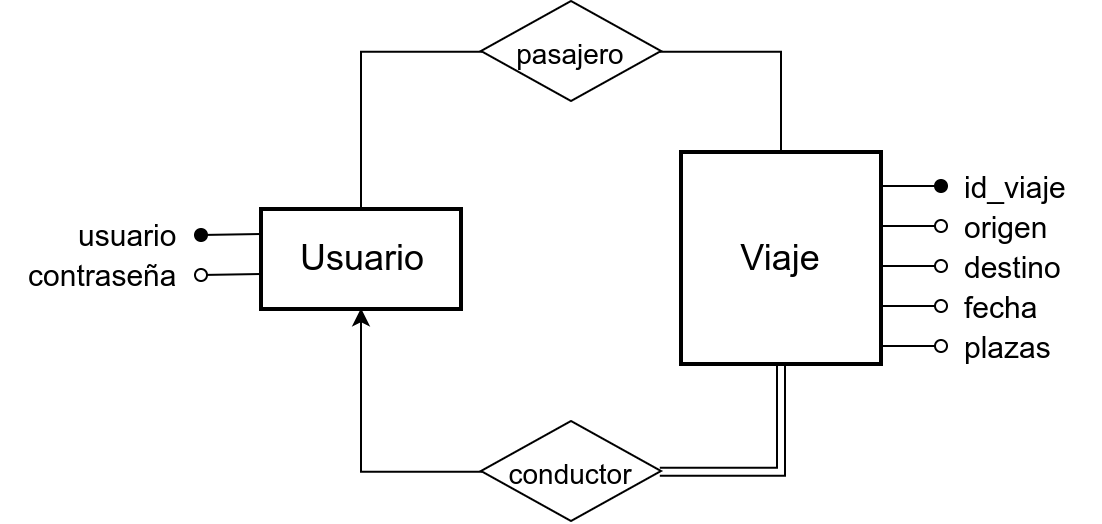
\includegraphics[width=10cm]{./../Graficas/db.png}
\end{center}


\section{Clases de la aplicación}

La aplicación utiliza las siguientes clases:
\vspace{-0.2cm}

\begin{itemize}
	\item \texttt{\textbf{ProcesadorCarriCar}}, que, ejecutada por el servidor, realiza las operaciones que manipulan y extraen información de la base de datos, resolviendo de este modo las peticiones del cliente.\vspace{-0.2cm}
	\item \texttt{\textbf{CarriCarInfoViaje}}, clase auxiliar para representar la información de un viaje.\vspace{-0.2cm}
	\item \texttt{\textbf{CarriCarDB}}, que contiene los métodos encargados de resolver peticiones a la base de datos \emph{SQLite} almacenada, por defecto, en \texttt{db/carricar\_database.db}.\vspace{-0.2cm}
	\item \texttt{\textbf{CarriCarStatus}}, clase \texttt{enum} usada para distinguir los estados en los que se encuentra el cliente.\vspace{-0.2cm}
	\item \texttt{\textbf{CarriCarClienteTCP}}, que contiene los métodos y el \texttt{main} que ejecuta el proceso cliente.\vspace{-0.2cm}
	\item \texttt{\textbf{CarriCarServidorIterativo}}, que contiene los métodos y el \texttt{main} que ejecuta el proceso servidor.\vspace{-0.2cm}
\end{itemize}

\pagebreak

\part{Diagrama de estados del servidor}

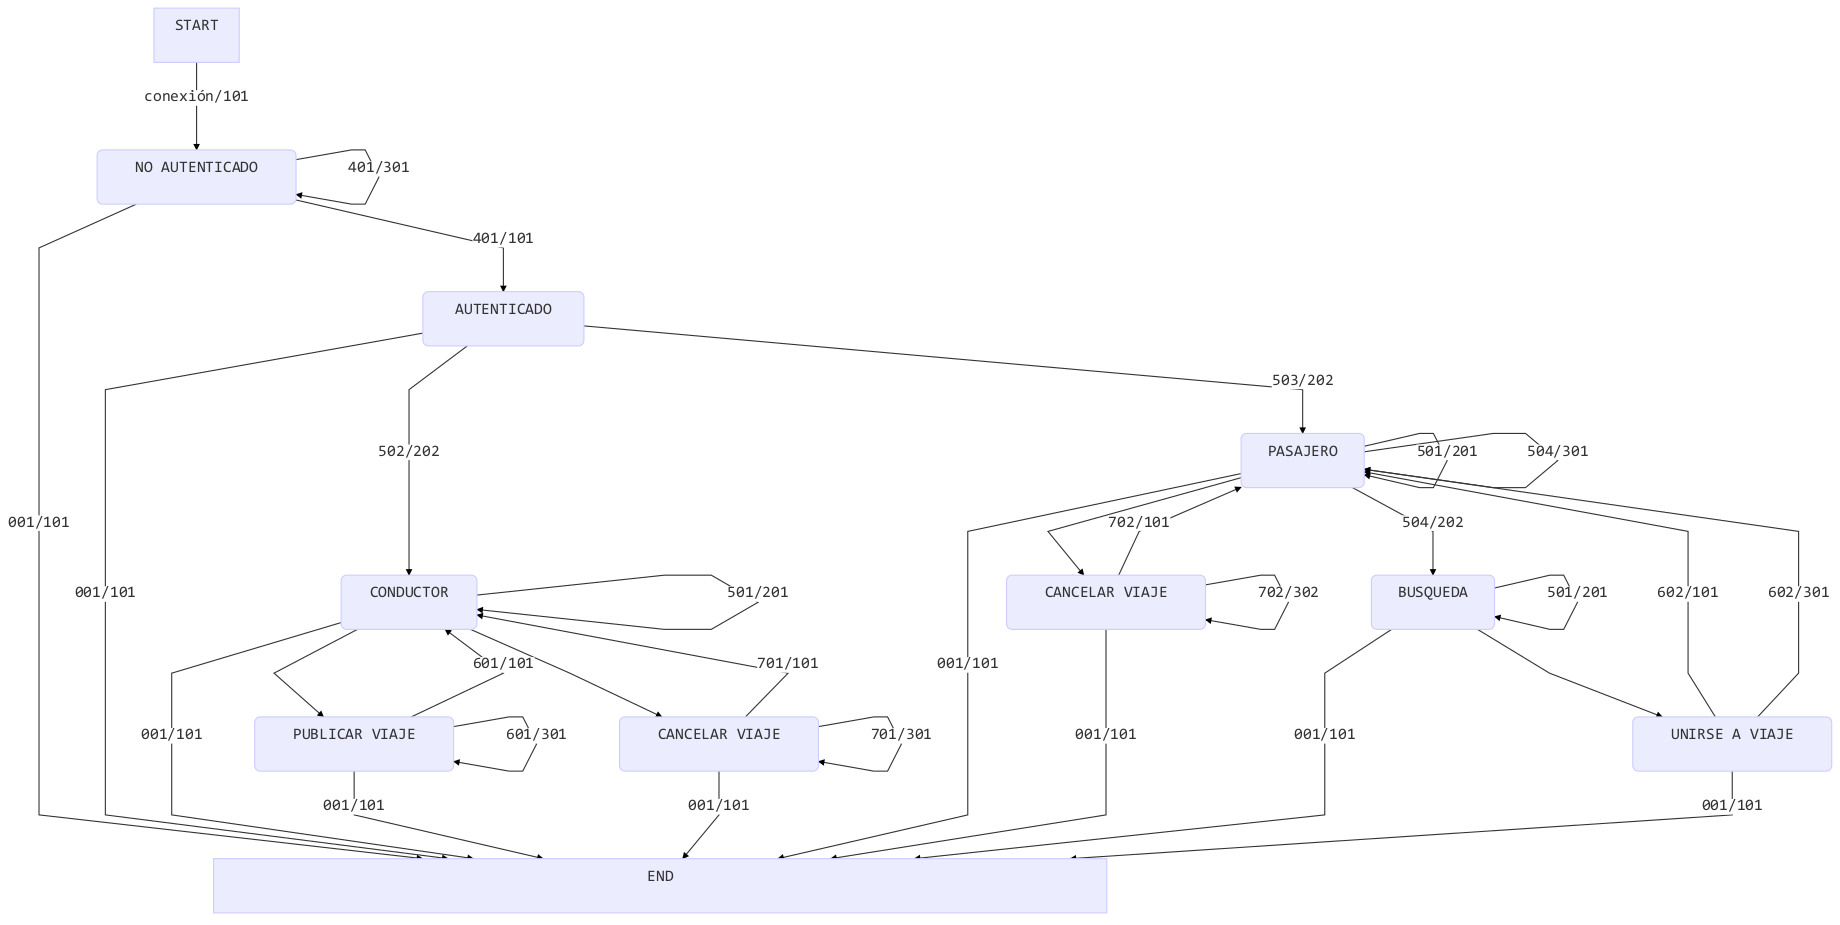
\includegraphics[width=15cm]{./../Graficas/diagram.png}
\hspace*{2cm}
\begin{table}[h]
\begin{tabular}{|C{2.5cm}|C{2.5cm}|L{9.7cm}|}
\multicolumn{1}{c}{}&\multicolumn{1}{c}{}&\multicolumn{1}{c}{}\\
\hline
\multicolumn{1}{|c}{\cellcolor[HTML]{81c784}\textbf{Cód. recibido}} & \multicolumn{1}{|c}{\cellcolor[HTML]{81c784}\textbf{Cód. enviado}} & \multicolumn{1}{|c|}{\cellcolor[HTML]{81c784}\textbf{Descripción}}\\
\hline
Conexión TCP & 101 & El cliente se conecta al servidor, y éste le saluda \\
\hline
* & 301 & El mensaje recibido no se corresponde con ninguno de los especificados \\
\hline
401 & 101 & El usuario inicia correctamente sesión en la aplicación \\
\hline
401 & 301 & El usuario no inicia correctamente sesión en la aplicación \\
\hline
501 & 201 & El cliente solicita información de un viaje, y el servidor le responde con dicha información \\
\hline
501 & 301 & El cliente solicita información de un viaje inexistente, el servidor envía un mensaje de error \\
\hline
502 & 202 & El cliente solicita los viajes de los que un usuario es conductor, y el servidor responde con la lista de dichos viajes \\
\hline
502 & 301 & El cliente solicita los viajes de los que un usuario inexistente es conductor, y el servidor responde con un mensaje de error \\
\hline
503 & 202 & El cliente solicita los viajes de los que un usuario es pasajero, y el servidor responde con la lista de dichos viajes \\
\hline
503 & 301 & El cliente solicita los viajes de los que un usuario inexistente es pasajero, y el servidor responde con un mensaje de error \\
\hline
504 & 202 & El cliente solicita una búsqueda de viajes junto a cierto criterio, y el servidor responde con la lista de dichos viajes, pudiendo estar dicha lista vacía \\
\hline
504 & 301 & El cliente solicita una búsqueda de viajes junto a cierto criterio, y el servidor no es capaz de completar la petición \\
\hline
\end{tabular}
\end{table}

\begin{table}[h]
\begin{tabular}{|C{2.5cm}|C{2.5cm}|L{9.7cm}|}
\hline
\multicolumn{1}{|c}{\cellcolor[HTML]{81c784}\textbf{Cód. recibido}} & \multicolumn{1}{|c}{\cellcolor[HTML]{81c784}\textbf{Cód. enviado}} & \multicolumn{1}{|c|}{\cellcolor[HTML]{81c784}\textbf{Descripción}}\\
\hline
601 & 101 & El cliente solicita la creación de un viaje, y el servidor lo crea satisfactoriamente \\
\hline
601 & 301 & El cliente solicita la creación de un viaje, y el servidor no lo crea porque el formato es incorrecto o porque la fecha es anterior a la actual \\
\hline
602 & 101 & El cliente solicita formar parte de un viaje, y el servidor completa la petición satisfactoriamente \\
\hline
602 & 301 & El cliente solicita formar parte de un viaje, y el servidor no es capaz de completar la petición por ser el viaje o el usuario inexistentes, o por no tener plazas disponibles \\
\hline
701 & 101 & El cliente solicita cancelar un viaje del que es conductor, y el servidor lo cancela satisfactoriamente \\
\hline
701 & 301 & El cliente solicita cancelar un viaje del que es conductor, y el servidor no puede hacerlo por ser el usuario o el viaje inexistentes, o por no ser el usuario conductor del viaje especificado \\
\hline
702 & 101 & El cliente solicita dejar de formar parte de un viaje como pasajero, y el servidor realiza la petición satisfactoriamente \\
\hline
702 & 301 & El cliente solicita dejar de formar parte de un viaje como pasajero, y el servidor no es capaz de completar la petición por no existir el usuario o el viaje, o no ser el usuario pasajero del viaje \\
\hline
001 & 101 & El cliente solicita cerrar sesión, y el servidor se despide \\
\hline
\end{tabular}
\end{table}
\hspace{1cm}

\pagebreak


\part{Mensajes que intervienen}

\begin{datos}
	{\bf\sffamily \hspace{-0.2cm} Nota.} {En el cuerpo se usa un separador, ``|'', que en el caso de nuestra aplicación es ``\texttt{@}''.}
\end{datos}

\section{Cliente}

\begin{table}[h]
\begin{tabular}{|C{1.2cm}|L{4.5cm}|L{9cm}|}
\hline
\multicolumn{1}{|c}{\cellcolor[HTML]{81c784}\textbf{Código}} & \multicolumn{1}{|c}{\cellcolor[HTML]{81c784}\textbf{Cuerpo}} & \multicolumn{1}{|c|}{\cellcolor[HTML]{81c784}\textbf{Descripción}}\\
\hline
401 & \texttt{usuario} | \texttt{contrasenia} & \textbf{Mensaje de autenticación.} Mensaje enviado por el cliente para iniciar sesión en la aplicación \\
\hline
501 & \texttt{id\_viaje} & \textbf{Solicitud de información de viaje.} Mensaje enviado por el cliente para recibir información sobre el viaje \\
\hline
502 & \texttt{usuario\_conductor} & \textbf{Solicitud de viajes conductor.} Mensaje enviado por el cliente para recibir los viajes de los que el usuario \texttt{usuario\_conductor} es conductor \\
\hline
503 & \texttt{usuario\_pasajero} & \textbf{Solicitud de viajes pasajero.} Mensaje enviado por el cliente para recbir los viajes de los que el usuario \texttt{usuario\_pasajero} es pasajero \\
\hline
504 & \texttt{origen} | \texttt{destino} & \textbf{Solicitud de búsqueda.} Mensaje enviado por el cliente para buscar viajes disponibles de acuerdo a los criterios de búsqueda especificados en el cuerpo \\
\hline
601 & \texttt{origen} | \texttt{destino} | \texttt{fecha} | \texttt{no\_plazas} | \texttt{usuario\_conductor} & \textbf{Solicitud de creación de viaje.} Mensaje enviado por el cliente para solicitar la creación de un viaje del que \texttt{usuario\_conductor} es conductor, de acuerdo a los parámetros especificados en el cuerpo \\
\hline
602 & \texttt{id\_viaje} | \texttt{usuario\_pasajero} & \textbf{Solicitud para formar parte como pasajero.} Mensaje enviado por el cliente para solicitar que el usuario \texttt{usuario\_pasajero} forme parte del viaje \texttt{id\_viaje} como pasajero \\
\hline
701 & \texttt{id\_viaje} & \textbf{Solicitud de cancelación de viaje conducido.} Mensaje enviado por el cliente para solicitar la cancelación del viaje \texttt{id\_viaje} (por el conductor de éste) \\
\hline
702 & \texttt{id\_viaje} | \texttt{usuario\_pasajero} & \textbf{Solicitud de cancelación de viaje por pasajero.} Mensaje enviado por el cliente para solicitar la cancelación de formar parte del viaje \texttt{id\_viaje} por parte del pasajero \texttt{usuario\_pasajero}.\\
\hline
001 & & \textbf{Solicitud de salida.} Mensaje enviado por el cliente para notificar de que el usuario quiere salir de la aplicación. \\
\hline

\end{tabular}
\end{table}

\pagebreak
\section{Servidor}

\begin{table}[h]
\begin{tabular}{|C{1.2cm}|L{4.5cm}|L{9cm}|}
\hline
\multicolumn{1}{|c}{\cellcolor[HTML]{81c784}\textbf{Código}} & \multicolumn{1}{|c}{\cellcolor[HTML]{81c784}\textbf{Cuerpo}} & \multicolumn{1}{|c|}{\cellcolor[HTML]{81c784}\textbf{Descripción}}\\
\hline
101 & \texttt{\emph{Mensaje de confirmación}} & \textbf{Respuesta de confirmación.} Mensaje enviado por el servidor para indicar que la solicitud ha sido efectuada correctamente \\
\hline
201 & \texttt{id\_viaje} | \texttt{origen} | \texttt{destino} | \texttt{fecha} | \texttt{no\_plazas} | \texttt{usuario\_conductor} | \texttt{usuario\_pasajero-1} | ... | \texttt{usuario\_pasajero-n} & \textbf{Respuesta con información de viaje.} Mensaje enviado por el servidor con la información del viaje \texttt{id\_viaje} \\
\hline
202 & \texttt{id\_viaje-1} | ... | \texttt{id\_viaje-n} & \textbf{Respuesta con conjunto de viajes.} Mensaje enviado por el servidor con una lista de viajes, identificados por su \texttt{id\_viaje} \\
\hline
301 & \texttt{\emph{Mensaje de error}} & \textbf{Respuesta de error.} Mensaje enviado por el servidor para indicar que ha habido algún error resolviendo la petición \\
\hline
\end{tabular}
\end{table}

\pagebreak

\part{Evaluación de la aplicación}

Tanto el servidor como el cliente están escritos en Java, basta ejecutar por separado los \texttt{main} de las clases \texttt{CarriCarServidorIterativo} y \texttt{CarriCarClienteTCP}.

En la aplicación hay incorporados diversos usuarios. Utilice el usuario \texttt{usuario} y contraseña \texttt{usuario} para iniciar sesión.

A continuación una captura de pantalla de la ejecución en el cliente:

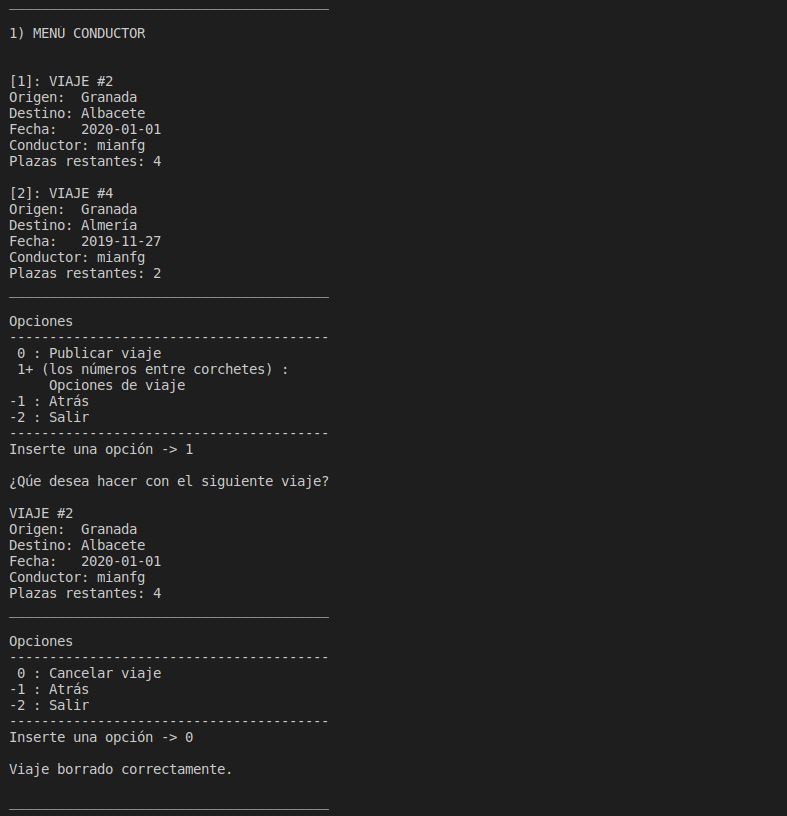
\includegraphics[width=15cm]{./../Graficas/clientcapture.png}

\pagebreak
Así como de los mensajes que recibe y envía el servidor:

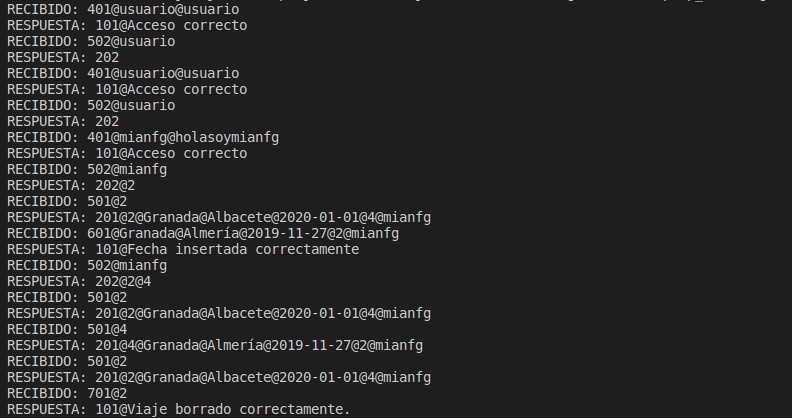
\includegraphics[width=15cm]{./../Graficas/servercapture.png}

Adjunto a este documento están los archivos \texttt{client\_log.txt} y \texttt{server\_log.txt}, que son el output de una sesión de uso de la aplicación.
\end{document}
 